%\PassOptionsToPackage{capitalize,noabbrev,nameinlink}{cleveref}                                                                                                                                                 
%\PassOptionsToPackage{usenames,dvipsnames}{color}
% \PassOptionsToPackage{numbers,compress,sort}{natbib}
\documentclass[11pt,times]{article}
\usepackage{submissions/selfdriving/deauther}
\usepackage{submissions/selfdriving/debulletin}

\newcommand{\paperTitle}{External vs. Internal: An Essay on\texorpdfstring{\\}{}
        Machine Learning Agents for\texorpdfstring{\\}{}
        Autonomous Database Management Systems}
\newcommand{\paperKeywords}{Self-Driving Databases, Autonomous Databases, Machine Learning for 
Databases, VGltS3Jhc2thQmV0cmF5ZWRNZQo=}
\newcommand{\paperAuthors}{Andrew Pavlo, Matthew Butrovich, Ananya Joshi, Lin Ma, Prashanth 
Menon, Dana Van Aken, Lisa Lee, Ruslan Salakhutdinov}

%% ==================================================================
%% PACKAGES
%% ==================================================================

%\setlength{\paperheight}{11in}
%\setlength{\paperwidth}{8.5in}

% hyperref itself
%\usepackage[
%            bookmarks=true, 
%%            colorlinks=true, 
%            bookmarksopen=true, 
%            pdfhighlight=/I,
%            pdfpagemode=UseOutlines, 
%            linkcolor=blue, 
%            pdfborder={ 0 0 0 },
%            pageanchor=false]{hyperref}
%\hypersetup{
%    pdfauthor = {\paperAuthors},
%    pdftitle = {\paperTitle},
%    pdfkeywords = {\paperKeywords},
%    pdfborder={ 0 0 0 }
%}
\usepackage{hyperref}
%\hypersetup{
%    colorlinks=true,
%    linkcolor=blue,
%    filecolor=magenta,      
%    urlcolor=cyan,
%}
\usepackage{amsmath}
\usepackage{amssymb}
\usepackage{boxedminipage}
\usepackage{xspace}
\usepackage{tabularx}
\usepackage{balance}  % for  \balance command ON LAST PAGE  (only there!)
%\usepackage[hyphenbreaks]{breakurl}
%\usepackage[font={small}]{caption}
\usepackage{graphicx}
\usepackage{subfig}
%\usepackage[usenames,table]{xcolor}
\usepackage{cleveref}
\usepackage{tabularx}
\usepackage{deauthor}
\usepackage{epsfig}

% \newcommand*{\newblock}{}
%\usepackage[numbers,sort]{natbib}
%\setlength{\bibsep}{6pt plus 0.3ex}

% font selection
\usepackage{times}
%\usepackage[final]{microtype}
%\usepackage[scaled]{inconsolata}
%\usepackage[T1]{fontenc}
\usepackage{graphicx}
\usepackage{subfig}
\usepackage{soul}
\usepackage{pifont}

% standard packages that must be loaded after hyperref
\usepackage{booktabs}
%\usepackage[end]{algpseudocode}
\usepackage{algorithm}

% cleveref goes last to get alg name right
\newcommand{\algorithmname}{Algorithm}
\newcommand{\theoremname}{Theorem}
\newcommand{\definitionname}{Definition}
\newcommand{\lemmaname}{Lemma} 

% captions
%\captionsetup{font=small}
%\captionsetup{labelfont=bf}
%\captionsetup[subfloat]{font=scriptsize}
%\captionsetup[subfloat]{farskip=5pt}
%\captionsetup[subfloat]{captionskip=1pt}
%\captionsetup[table]{belowskip=0pt}

%\captionsetup[table]{position=t}
%\captionsetup[table]{skip=\medskipamount}

% captions placed on the bottom for figures
%\captionsetup[figure]{position=b}
%figures and tables numbered by section
%\captionsetup{figurewithin=section}
%\captionsetup{tablewithin=section}

\clubpenalty=10000
\widowpenalty = 10000

\newcommand{\tabitem}{\textbullet~}

% multi-line in table
\newcommand{\mlbegin}{\shortstack\bgroup}
\newcommand{\mlend}{\egroup}

%% Squished Lists
\newcommand{\squishitemize}{
 \begin{list}{$\bullet$}
  { \setlength{\itemsep}{0pt}
     \setlength{\parsep}{3pt}
     \setlength{\topsep}{3pt}
     \setlength{\partopsep}{0pt}
     \setlength{\leftmargin}{1.95em}
     \setlength{\labelwidth}{1.5em}
     \setlength{\labelsep}{0.5em} } }

\newcounter{Lcount}
\newcommand{\squishlist}{
    \begin{list}{\arabic{Lcount}. }
   { \usecounter{Lcount}
        \setlength{\itemsep}{0pt}
        \setlength{\parsep}{3pt}
        \setlength{\topsep}{3pt}
        \setlength{\partopsep}{0pt}
        \setlength{\leftmargin}{2em}
        \setlength{\labelwidth}{1.5em}
        \setlength{\labelsep}{0.5em} } }

\newcommand{\squishend}{\end{list}}

\definecolor{todo-color}{rgb}{1,0,0}
\newcommand{\todo}[1]{\textnormal{\color{todo-color}{\textbf{#1}}}\unskip}

\definecolor{comment-color}{rgb}{0.25,0.25,0.25}
\newcommand{\codeComment}[1]{\textnormal{\color{comment-color}{\textit{\textbf{\# #1}}}}\unskip}

%% ==================================================================
%% MAGIC FIGURE SPACING
%% ==================================================================

% Single-Column Figures
\setlength{\floatsep}{5pt}
\setlength{\textfloatsep}{5pt}
\setlength{\abovecaptionskip}{0.5em}
\setlength{\belowcaptionskip}{0.5em}

% % Multi-Column Figures
\setlength{\dbltextfloatsep}{5pt}
\setlength{\dblfloatsep}{5pt}

% Subfigures
% \setlength{\subfigcapskip}{0in}
% \setlength{\subfigtopskip}{0pt}
% \setlength{\subfigbottomskip}{2pt}

%% ==================================================================
%% MACROS
%% ==================================================================

% Database Stuff
\newcommand{\dbSQL}[1]{\texttt{\textbf{#1}}\xspace}
\newcommand{\dbKnob}[1]{\texttt{#1}\xspace}
\newcommand{\dbKnobFootnote}[2]{\footnote{\scriptsize{#1 Knob -- \texttt{#2}}}}

%% OTTERTUNE
% Database Systems
\newcommand{\ottertune}{OtterTune\xspace}
\newcommand{\toolName}{OtterTune\xspace}
\newcommand{\toolNameS}{OtterTune's\xspace}
\newcommand{\knobBase}{knob}
\newcommand{\knob}{\knobBase\xspace}
\newcommand{\knobs}{\knobBase{s}\xspace}
\newcommand{\KnobBase}{Knob}
\newcommand{\Knob}{\KnobBase\xspace}
\newcommand{\Knobs}{\KnobBase{s}\xspace}
\newcommand{\KNOBBASE}{KNOB}
\newcommand{\KNOB}{\KNOBBASE\xspace}
\newcommand{\KNOBS}{\KNOBBASE{S}\xspace}
\newcommand{\metricBase}{metric}
\newcommand{\metric}{\metricBase\xspace}
\newcommand{\metrics}{\metricBase{s}\xspace}
\newcommand{\MetricBase}{Metric}
\newcommand{\Metric}{\MetricBase\xspace}
\newcommand{\Metrics}{\MetricBase{s}\xspace}
\newcommand{\METRICBASE}{METRIC}
\newcommand{\METRIC}{\METRICBASE\xspace}
\newcommand{\METRICS}{\METRICBASE{S}\xspace}


\newcommand{\dbmsMySQL}{MySQL\xspace}
\newcommand{\dbmsPostgres}{Postgres\xspace}
\newcommand{\toolClient}{controller\xspace}
\newcommand{\toolServer}{tuning manager\xspace}
\newcommand{\toolRepo}{repository\xspace}

%% CMU-DB
\newcommand{\noisepage}{NoisePage\xspace}

%% ==================================================================
%% DOCUMENT
%% ==================================================================
\begin{document}

\newcommand{\mail}[1]{\href{mailto:#1}{#1}}

\title{External vs. Internal: An Essay on Machine Learning Agents for Autonomous Database Management Systems}

%\author{
%    \href{mailto:pavlo@cs.cmu.edu}{Andrew Pavlo},
%    \href{mailto:mbutrovi@cs.cmu.edu}{Matthew Butrovich},
%    \href{mailto:aajoshi@cs.cmu.edu}{Ananya Joshi},
%    \href{mailto:lin.ma@cs.cmu.edu}{Lin Ma},
%    \href{mailto:pmenon@cs.cmu.edu}{Prashanth Menon},
%    \href{mailto:dvanaken@cs.cmu.edu}{Dana Van Aken} \\
%    \href{mailto:lslee@cs.cmu.edu}{Lisa Lee},
%    \href{mailto:rsalakhu@cs.cmu.edu}{Ruslan Salakhutdinov} \\
%    \textit{Carnegie Mellon University} \\
%    {\{ 
%        \href{mailto:pavlo@cs.cmu.edu}{pavlo},
%        \href{mailto:mbutrovi@cs.cmu.edu}{mbutrovi},
%        \href{mailto:aajoshi@cs.cmu.edu}{aajoshi},
%        \href{mailto:lin.ma@cs.cmu.edu}{lin.ma},
%        \href{mailto:pmenon@cs.cmu.edu}{pmenon},
%        \href{mailto:dvanaken@cs.cmu.edu}{dvanaken},
%        \href{mailto:lslee@cs.cmu.edu}{lslee},
%        \href{mailto:rsalakhu@cs.cmu.edu}{rsalakhu}
%    \}@cs.cmu.edu}
%}
\author{Andrew Pavlo\(^1\), Matthew Butrovich\(^1\), Ananya Joshi\(^1\), Lin Ma\(^1\),\\ Prashanth Menon\(^1\), Dana Van Aken\(^1\), Lisa Lee\(^1\),Ruslan Salakhutdinov\(^1\),\\
\(^1\)Carnegie Mellon University}

\maketitle

%% ==================================================================
%% ABSTRACT
%% ==================================================================
\begin{abstract}
The limitless number of possible ways to configure database management systems (DBMSs) has 
rightfully earned them the reputation of being difficult to manage and tune.
% Studies have shown that DBAs spend nearly 25\% of their time on 
% tuning activities~\cite{debnath08} and personnel is estimated to be 50\% of a DBMS's total 
% cost~\cite{rosenberg06}.
Optimizing a DBMS to meet the needs of an application has surpassed the 
abilities of humans. This is because the correct configuration of a DBMS is highly 
dependent on a number of factors that are beyond what humans can reason about. The problem is 
further exacerbated in large-scale deployments with thousands or even millions of individual DBMS 
installations that each have their own tuning requirements.
    
To overcome this problem, recent research has explored using machine learning-based (ML) agents 
for automated tuning of DBMSs. These agents extract performance metrics and behavioral 
information from the DBMS and then train models with this data to select 
tuning actions that they predict will have the most benefit. They then observe how 
these actions affect the DBMS and update their 
models to further improve their efficacy.

In this paper, we discuss two engineering approaches for integrating ML agents 
in a DBMS. The first is to build an external tuning controller that treats the DBMS as a black-box. 
The second is to integrate the ML agents natively in the DBMS's architecture.
We consider the trade-offs of these approaches in the context of two projects from 
Carnegie Mellon University (CMU). 

\end{abstract}

%% ==================================================================
%% INTRODUCTION
%% ==================================================================
\section{Introduction}
\label{sec:introduction}
Tuning a DBMS is an essential part of any database application 
installation. The goal of this tuning is to improve a DBMS's operations based on some 
objective function (e.g., faster execution, lower costs, better availability). Modern DBMSs provide 
APIs that allow database administrators (DBAs) to control their runtime execution and storage
operations: (1) \textit{physical design}, (2) \textit{knob configuration}, (3) \textit{hardware 
resource allocation}, and (4) \textit{query plan hints}. The first are changes to the database's 
physical representation and data structures 
(e.g., indexes, views, partitioning). The second are optimizations that 
affect the DBMS's behavior through its configuration knobs (e.g., caching policies).
Resource allocations determine how the DBMS uses its available hardware to store data and execute 
queries; the DBA can either provision new resources (e.g., adding disks, 
memory, or machines) or redistribute existing resources (e.g., partitioning tables across 
disks). Lastly, query plan 
tuning hints are directives that force the DBMS's optimizer to make certain decisions 
for individual queries (e.g., join orderings).

Given the notorious complexity of DBMS tuning, a reoccurring theme in 
database research over the last five decades has been on how to automate this process and reduce 
the burden on humans.
The first efforts in the 1970s were on building \textit{self-adaptive} systems~\cite{hammer77}. 
These were primarily recommendation tools that focused on physical database design (e.g, 
indexes~\cite{hammer76,hudson89}, partitioning~\cite{hammer79,levin82}, clustering~\cite{yu85}). 
They were also external to the DBMS and meant to assist the DBA with the tuning process.
In the 1990s, the database community switched to using the moniker \textit{self-tuning} 
systems~\cite{chaudhuri07,weikum94}. Like their predecessors, most of the self-tuning systems 
targeted automated physical design~\cite{gupta97,chaudhuri97,valentin00}. But they also expanded 
their scope to include automatic DBMS knob configuration~\cite{sullivan04,debnath08,tian03}. 
This was necessary because by then the more mature DBMSs had hundreds of tunable 
knobs and the problem of how to set them correctly because too arduous~\cite{vanaken17}.
Another notable difference was that while most of the self-adaptive methods were primarily in 
the context of standalone recommendation 
tools that were external to the DBMS, some vendors added self-tuning components 
directly inside of the DBMS~\cite{kwan02,storm06,dageville02}.

The current research trend is on how to use of machine learning (ML) to devise 
``learned'' methods for automated DBMS tuning. 
Instead of relying on static heuristics or cost models (see Section~\ref{sec:background}), these newer 
approaches train models using data collected about the DBMS's runtime behavior under various 
execution scenarios and configurations. The tuning \textit{agent} then predicts the expected benefit 
of \textit{actions} (e.g., add an index) using these models and selects the one with the greatest 
expected reward. The agent then observes the affects of the deployed action and integrates this new 
data 
back into the models to improve their efficacy for future decision making.
This last step removes the need for a human to make judgment calls about whether or not to make a 
recommended change.

There are two ways developers can integrate such ML-based tuning methods for DBMSs. The first is to 
use external agents that observe and manipulate a DBMS through standard 
APIs (e.g., JDBC, ODBC). This approach is ideal for existing DBMSs where the 
software engineering effort required to retrofit the architecture to support automated tuning is 
too onerous. The second is to integrate internal components that directly operate inside of the 
DBMS. Building the ML components inside of the system obviates several problems 
related to training data collection and modeling, as well as enables the agent to have fine-grained 
control of the system's behavior. But this integration requires such a tight coupling that it is 
often only viable for those organizations that are designing a new system from 
scratch (i.e., a ``greenfield'' project)~\cite{pavlo19}.

In this paper, we discuss the trade-offs between implementing ML-based tuning agents outside of the 
DBMS versus designing a new DBMS around automation.
Our analysis is based on our experiences developing 
ML-based tuning tools for existing systems~\cite{vanaken17,zhang18-ottertune,pavlo12} and new 
autonomous architectures~\cite{arulraj16,ma18,pavlo17,pavlo11,zhang18-icde}.
We begin in Section~\ref{sec:background} with an overview of how DBMS tuning algorithms work. Next, in 
Section~\ref{sec:ml} we describe how to use ML-based agents to automatically tune systems.
We then compare the benefits of the approaches, as well as discuss 
some of their challenges and unsolved problems.
We conclude with an overview of two DBMS projects at CMU~\cite{cmu-db} on using ML 
for automated tuning. The first is \textbf{\ottertune}~\cite{ottertune}, an external knob tuning 
service for existing DBMSs. The other is a new self-driving~\cite{pavlo17} DBMS called 
\textbf{\noisepage}~\cite{noisepage} (formerly Peloton\footnote{We are unable to continue with 
    the Peloton~\cite{peloton} project due to the unholy combination of engineering, legal, and 
marital problems.}) that we are designing to be 
completely autonomous.

%% ==================================================================
%% BACKGROUND
%% ==================================================================
\section{Background}
\label{sec:background}
Previous researchers in the last 50 years have studied and devised several methods for 
automatically optimizing DBMSs~\cite{bernstein98,chaudhuri00,chaudhuri07,weikum02}. As such, there 
is an extensive corpus of previous work, including both theoretical~\cite{ceri83} and applied 
research~\cite{duan09,zilio04,wiese08}.
Before the 2010s, the core methodologies for automated DBMS tuning were
either (1) heuristic- or (2) cost-based optimization algorithms. We now briefly discuss this prior 
work to motivate the transition to ML-based methods in Section~\ref{sec:ml}.

The most widely used approach in automated DBMS tuning is to use \textit{heuristic} algorithms 
that are comprised of hard-coded rules that recommend 
actions~\cite{hammer79}. For example, IBM's first release of their 
DB2 Performance Wizard tool in the early 2000s asked the DBA questions about their application 
(e.g., whether it is 
OLTP or OLAP) and then provides knob settings based on their answers~\cite{ibmdb02}. It uses rules 
manually created by DB2 engineers and thus may not accurately reflect the actual workload or 
operating environment. IBM 
later released a version of DB2 with a self-tuning memory manager that again uses rules to 
determine how to allocate the DBMS's memory to its internal components~\cite{storm06,tian03}. 
Oracle has a similar ``self-managing'' memory manager in their DBMS~\cite{dageville02}, but also 
provides a tool to identify bottlenecks due to misconfiguration using rules~\cite{dias05,kumar03}.
Others have used the same approach in tuning tools for Microsoft's SQL 
Server~\cite{narayanan05}, MySQL~\cite{mysql-tuning-primer}, and Postgres~\cite{postgres-pgtune}.

The other common approach for DBMS tuning is to use \textit{cost-based} algorithms that 
programmatically search for improvements to the DBMS's configuration. 
These algorithms are guided by a cost model that estimates the benefits of design choices based on 
a representative sample workload trace from the application. 
A cost model allows a tool to identify good actions without having to deploy them for real on the 
DBMS, which would is prohibitively expensive and slow.
Previous work in this area has evaluated several search techniques, including 
greedy search~\cite{chaudhuri97}, branch-and-bound search~\cite{pavlo12,zilio04,nehme11}, local 
search~\cite{xi04}, genetic algorithms~\cite{nehme11}, and relaxation/approximation~\cite{bruno05}. 

To avoid the problem of a cost-based algorithm making choices that do not reflect what happens in 
the real DBMS, the tuning tool can use the DBMS's internal components to provide it with more 
accurate cost model estimations. The 
first and most notable application of this optimization was Microsoft's AutoAdmin use of SQL 
Server's built-in cost models from its query planner to estimate 
the utility of indexes~\cite{chaudhuri98}.
Relying on the DBMS for the cost model, however, does not work for knob configuration tuning 
algorithms. In the case of Microsoft's example of using the query planner to guide its search 
algorithms, these models approximate on the amount of work to execute a query and 
are intended to compare alternative query execution strategies in a fixed 
environment~\cite{soror08}. But knobs affect a DBMS's behavior in ways that are not easily reflected 
(if even possible) in the query planner's cost model. For example, it is non-trivial for the 
planner 
to reason for a single query about a knob that changes caching policies since the behavior can vary 
depending on the 
workload. Hence, the major vendors' proprietary knob configuration tools mostly rely on static 
heuristics and vary in the amount of automation that they 
support~\cite{dias05,kumar03,narayanan05,mysql-tuning-primer,postgres-pgtune}.

The critical limitation in both of the above heuristic- and cost-based tuning methods is that they 
tune each DBMS in isolation. That is, they only reason about how to tune one particular DBMS 
instance and do not leverage information collected about previous tuning sessions.
Heuristic-based methods rely on assumptions about the DBMS's workload and environment that may not 
accurately reflect the real-world.
The lack of data reuse increases the amount of time that it takes for cost-based algorithms to find 
improvements for the DBMS. To avoid an exhaustive search every time, developers apply domain 
knowledge about databases to prune the solutions that are unlikely to provide any benefit. For 
example, an index selection algorithm can ignore candidate indexes for columns that are never 
accessed in queries. But database tuning problems are NP-Complete~\cite{mukkamala88,ip83}, and thus 
solving them efficiently even with such optimizations is non-trivial. This is where ML-based 
approaches can potentially help by providing faster approximations for optimization problems.

%% ==================================================================
%% Automated Tuning with ML 
%% ==================================================================
\section{Automated Tuning with Machine Learning}
\label{sec:ml}
ML is a broad field of study that encompasses many disciplines and is applicable to many facets of 
DBMSs. There are engineering and operational challenges in incorporating 
ML-based components into already complex DBMS software stacks~\cite{sculley14}, such as 
explainability, maintainability/extendability, and stability. 
There are also important problems on automatically provisioning resources for a fleet of DBMSs in a 
cloud environment. We limit the scope of 
our discussion to the implications 
of integrating ML in DBMSs for tuning in either existing or new system architectures.

ML-based agents for automated DBMS tuning use algorithms that rely on 
statistical models to select actions that improve the system's target objective. 
That is, instead of being provided explicit instructions on how to tune the DBMS, the agent 
extracts patterns and inferences from the DBMS's past behavior to predict the 
expected behavior in the future to lean how to apply it to new actions.
The agent selects an action that it believes will provide the most benefit to its target objective 
function. It then deploys this action without having to request permission from a DBA. This 
deployment can either be explicit (e.g., invoking a command to build an index) or 
implicit (i.e., updating its models so that the next invocation reflects the change).

Agents build their models from training data that they collect from the DBMS and its 
environment. This data can also come from other previous tuning sessions for other DBMSs 
if they provide the proper context (e.g., hardware profile).
The type of data that an agent collects from the DBMS depends on its action domain. Some agents 
target a specific sub-system in the DBMS, and thus they need training data related to these 
parts of the system. For example, an agent that tunes the DBMS's query 
optimizer~\cite{marcus18,ortiz18} collects information about the workload (e.g., SQL queries) and 
the distribution of values in the database. Another agent that targets tuning the DBMS's knob 
configuration only needs low-level performance 
metrics as this data is emblematic of the overall behavior of the system for a 
workload~\cite{vanaken17,zhang19-cdbtune,duan09}.
A holistic tuning agent that seeks to control the entire DBMS collects data from every parts of the 
system because they must consider latent interactions between them~\cite{pavlo17}.

How an agent acquires this data depends on whether it trains its models offline or 
online. Offline training is where the agent replays a sample workload trace while varying the 
DBMS's configuration in a controlled environment.  This arrangement allows the agent to guide its 
training process to explore unknown regions in its solution space. Offline training also ensures 
that if the agent selects a bad configuration that it does not cause observable problems in the 
production environment.
With online training, the agent observes the DBMS's behavior directly as it executes the 
application's workload. This approach does not require the system to provide the agent a workload 
sample; this allows the agent to always have an up-to-date view of the workload. The agent, however, 
may cause the system to make unexpected changes that hurt performance and require a 
human to intervene. Note also that the offline versus online approaches are not mutually 
exclusive and a DBMS can use both of them together.

ML methods are divided into three broad categories: (1) \textit{supervised}, (2) 
\textit{unsupervised}, and (3) \textit{reinforcement learning}. There are existing DBMS tuning 
agents that use either one category of 
algorithms or some combination of them. We now describe these approaches in the context of DBMS 
tuning:
\\ \vspace{-0.1in}

%% -----------------------
%% Supervised Learning
%% -----------------------
\textbf{Supervised Learning:}
The agent builds models from training data that contains both the 
input and expected output (i.e., labels). The goal is for the models learn how to produce the 
correct answer for new inputs. This approach is useful for problems where the outcome of 
an action is immediately observable.
An example of a supervised learning DBMS tuning method is an algorithm that predicts the 
cardinality of query plan operators~\cite{ivanov17,liu15,woltmann19,kipf19}. The training data 
input contains encoded vectors of each operator's salient features (e.g., type, 
predicates, input data sizes) and the output is the cardinality that the DBMS observed when 
executing the query. The objective for this agent is to minimize the difference between the 
predicted and actual cardinalities.
Supervised learning has also been applied to tune other parts of a DBMS, including 
approximate indexes~\cite{kraska18}, performance modeling~\cite{ganapathi09,marcus19-perf}, 
transaction scheduling~\cite{pavlo11,sheng19}, query plan tuning~\cite{zhang19-ai}, and knob 
tuning~\cite{vanaken17}.
\\ \vspace{-0.1in}

%% -----------------------
%% Unsupervised Learning
%% -----------------------
\textbf{Unsupervised Learning:}
With this approach, the agent's training data only contains input values and not the expected 
output. It is up to the agent to infer whether the output from the models are correct. An example 
of this is an agent that clusters workloads into categories based on their access patterns
patterns~\cite{mozafari13,gupta08}. The assigned categories have no human decipherable meaning other 
than the workloads in each category are similar in some way. Although not directly related to 
tuning, another use of unsupervised ML in DBMSs is for automatically detecting data anomalies in a 
database: the agent does not need to be told what are ``correct'' values to figure out what 
values do not look like the others~\cite{bailis17}. 
\\ \vspace{-0.1in}

%% -----------------------
%% Reinforcement Learning
%% -----------------------
\textbf{Reinforcement Learning:}
Lastly, reinforcement learning (RL) is similar to unsupervised ML in that there is no labeled 
training data. The agent trains a policy model that selects actions that will improve the target 
objective function for the current environment. RL approaches in general do not make assumptions 
about priors and the models are derived only from the agent's observations. This is useful for 
problems where the benefit or effect of an action are not immediately known. For example, the agent 
may choose to add an index to improve query performance, but the DBMS will take several 
minutes or even hours to build it.
Even after the DBMS builds the index, the agent may still only observe its reward after a 
period of time if the queries that use do not come until later (e.g., due to workload pattern 
changes).
Given the general purpose nature of RL, it is one of the most active areas of DBMS tuning research 
in the late 2010s. Researchers have applied RL for query 
optimization~\cite{marcus18,ortiz18,marcus19-opt}, index 
selection~\cite{basu15,sharma18,zhang19-ai},
partitioning~\cite{durand18,hilprecht19}, and knob tuning~\cite{zhang19-cdbtune}.
\\ \vspace{-0.1in}

We next discuss how to integrate agents that use the above ML approaches into DBMSs 
to enable them to support autonomous tuning and optimization features. We begin with an examination 
of strategies for running agents outside of the DBMS in Section~\ref{sec:ml-external}. Then in 
Section~\ref{sec:ml-internal} we consider the implications of integrating the agents directly inside 
of the DBMS. For each of these strategies, we first present the high-level approach and then list 
some of the key challenges that one must overcome with them.

%% ---------------------------------------------------------------
%% Existing
%% ---------------------------------------------------------------
\subsection{External Agents}
\label{sec:ml-external}
An external agent tunes a DBMS without requiring specialized ML components running inside of the 
system. The goal is to reuse the DBMS's existing APIs and environment data collection 
infrastructure (e.g., query traces, performance metrics) without having to modify the DBMS itself 
or for the DBMS to be even aware that software and not a human is managing it.
Ideally a developer can create the agent in a general purpose such that one can reuse its backend 
ML component across multiple DBMSs.

% Most DBMS developers built their systems 
% under the assumption that humans will configure and manage them. Thus, an external tuning agent 
% uses an existing DBMS's APIs that are designed for humans to observe and interact with the system. 

An agent receives its objective function data either directly from the DBMS or through additional 
third-party monitoring tools (e.g., Prometheus, Druid, InfluxDB). The latter scenario is common in 
organizations with a large number of DBMS instances.
Although the agent's ML algorithms are not tailored to any particular DBMS, there is DBMS-specific 
code to prepare the training data for consumption by the algorithm. This is colloquially known as 
\textit{glue} code in ML parlance~\cite{sculley14}. 
For example, the agent has to encode configuration knobs with fixed ``enum'' values, 
known as a categorical variables, as separate one-hot 
encoded features since ML algorithms cannot operate on strings~\cite{vanaken17}. To do this encoding 
correctly, the agent must obviously be aware of all possible values a knob can take; it is too 
difficult and a waste of time to try to infer this on its own.

Agents may also need an additional \textit{controller} running on the same machine as the DBMS 
or within the same administrative domain~\cite{vanaken17}. This controller is allowed to install 
changes that are not accessible through the DBMS's APIs. For example, DBMSs that read configuration 
files at start-up on local disk will overwrite any previously set knob values. Thus, unless the 
agent is able to write these files, then it will not be able to persist changes. The controller 
may need to also restart the DBMS because many systems are not able to apply changes until 
after a restart.
\\ \vspace{-0.1in}

%% -----------------------
%% Challenges
%% -----------------------
\textbf{Challenges:}
There are several challenges in tuning an existing DBMS that was not originally designed for 
autonomous operation. Foremost is that almost every major DBMS that we have examined does not 
support 
making changes to the system's configuration without periods of unavailability, either due to 
restarts or blocking execution~\cite{pavlo19}. Requiring the DBMS to halt execution in order to 
apply a change makes it difficult for agents to explore 
configurations in production systems and increases the time it takes to collect training data.
There are methods for reducing start-up times~\cite{abraham13,graefe14}, but the agent still 
must also account for this time in their reward functions, which are often non-deterministic.

The second issue is that an agent is only able to collect performance metrics that 
the system already exposes. This means that if there is additional information that the agent 
needs, then it is not immediately available. The other issue is that is that there is often an 
overabundance of data that makes it difficult to 
separate signals from the noise~\cite{vanaken17}. Furthermore, DBMSs 
also do not expose information about their underlying hardware so the system can reuse 
training data across operating environments.
In many cases these metrics were originally meant to assist humans with 
diagnosing performance problems. That is, the developers added metrics 
assuming that they were meant for human consumption and not for enabling autonomous 
control. Many DBMSs do not report metrics at consistent intervals using the same unit of 
measurement.
% We have also found that some DBMS have incomplete metrics (i.e., missing 
% data for critical aspects of performance). These issues further complicate their usage 
% for training a ML model.

Lastly, every DBMS has knobs that requires human knowledge in order to know how to 
set it correctly. There are obvious cases, like knobs that define file paths or port numbers, where 
the system will not function if they are set incorrectly. But there are other knobs where if an 
agent sets it incorrectly then the system will not become inoperable; instead, they will subtly 
affect the database's correctness or safety. The most common example of this that we found is 
whether to require the DBMS to flush a 
transaction's log records to disk before it is committed. Turning off this flushing improves 
performance but may lead to data loss on failures.
If an agent discovers that 
changing this knob improves the objective function, then it will make that change. But the agent 
is unable to know what the right choice is because it requires a human to 
decide what is allowed in their organization. The agent's developers must mark such knobs as 
untunable in the glue code so that an agent do not modify them.

%% ---------------------------------------------------------------
%% Internal
%% ---------------------------------------------------------------
\subsection{Internal Agents}
\label{sec:ml-internal}
An alternative to treating the DBMS like a black-box and tuning it with an 
external agent is to design the system's architecture to natively
support autonomous operation. With this approach, the DBMS supports one or more 
agents running inside of the system. These agents collect their own training data, apply changes to 
the 
DBMS (ideally without restarting), and then observe how those changes affect the objective. The 
system does not require guidance or approval from a human for any of these steps.
The benefit of running agents inside of the DBMS is that it exposes more 
information about the system's runtime behavior and can potentially enable more low-level control 
of the DBMS than what is possible with an external agent.

Most of the proposed ML tuning agents that are available today are designed to extend or replace 
components in existing DBMSs. One of the first of these was IBM's 
Learning Optimizer from the early 2000s that used a feedback mechanisms to update 
the query planner's cost models with data that the system observed during from query 
execution~\cite{stillger01}. There are now more sophisticated proposals for changing the 
cost model with learned models to estimate cardinalities~\cite{ivanov17,liu15,woltmann19,kipf19} or 
even generate the query plan itself~\cite{ortiz18,marcus19}. These agents can also leverage the 
DBMS's existing components to help them ``bootstrap'' their models and provide them with a 
reasonable starting point.
% 
One notable example of augmenting an existing DBMS with ML agents is Oracle's cloud-based 
autonomous DBMS offering~\cite{oracle-selfdriving}. Although there is little public 
information about its implementation, our understanding from discussions with their developers is 
that it uses Oracle's previous independent tuning tools in a managed environment with limited 
centralized coordination.

Instead of augmenting an existing DBMS, others have looked into creating new DBMS 
architectures that are designed from the ground up for autonomous 
control~\cite{pavlo17,sharma18,kraska19}.
With a new system, the developers can tailor its implementation to make its components 
easier to model and control. They can also customize the architecture to be more 
friendly to automated agents (e.g., avoiding the need to restart the system when changing knobs, 
having a unified action deployment framework)~\cite{pavlo19}.
% We contend that one cannot create a fully autonomous DBMS architecture through independent 
% agents that are each tuning their own part of the system separately. Given this, some 
% have eschewed working with existing systems and seek to build new DBMSs that use ML 
% agents to control all aspects of its execution behavior. The difference with a new 
% architecture versus modifying an existing system is that a new system is able to 
% track the effect of actions across sub-systems and organizes its internal 
% information in a way that more amenable for consumption by algorithms instead 
% of humans~\cite{pavlo19}.
\\ \vspace{-0.1in}

%% -----------------------
%% Challenges
%% -----------------------
\textbf{Challenges:}
The biggest problem with replacing a DBMS's existing components with new ML-based implementations 
is that it is hard to capture the dependencies between them. That is, if each tuning agent 
operates under the assumption that the other parts of the system are fixed, then their
models will encapsulate this assumption. But then if each agent modifies their part of 
the DBMS that they control, then it will be hard to make accurate predictions. 
Consider a tuning agent that controls the DBMS's memory allocations. Suppose the 
agent initially assigns a small amount of memory for query result caching and a large amount to 
the buffer pool. Another index tuning agent running inside of the same DBMS then chooses to build 
an index because memory pressure 
in the buffer pool is low. But then the memory agent decides on its own to increase the result 
cache size and decrease the buffer pool size. With this change, there is now less memory available 
to store the index and data pages, thereby increasing the amount of disk I/O that the DBMS incurs 
during query execution. Thus, the index that the second agent just added is now a bad choice 
because of change in another part of the system that it does not control.

There are three possible ways to overcome this problem but each of them have their own set of 
issues. The first is to use a single centralized agent rather than separate agents. This 
is potentially the most practical but greatly increases the dimensionality (i.e., complexity) of 
the models, which requires significantly more training data. The second is to have each individual 
agent provide a 
performance guarantee about what its changes in the DBMS. The agents provide this information to 
a central coordinator that is in charge of resource allocations.
The last approach is to have a decentralized architecture where agents communicate and coordinate 
with each other. We suspect that this will prove to be too difficult to achieve reasonable 
stability or explainability.

% In all of these implementations, the agent will need to encode the DBMS's environment in their 
% models. But this increases the dimensionality of the models and may lead to unstable 
% performance. This environment encodes all aspects of the DBMS, including its (1) workload, 
% (2) hardware resources, (3) database design, (4) configuration, and (5) database 
% contents. Many of these components are variable length and dynamic. For example, 
% the number of possible indexes will change as the DBA adds/removes columns. The 
% large number of features in this environment also means that the agent needs a 
% significant amount of training data before the models can produce accurate and 
% meaningful results.

One of the most expensive parts of these agents is when they build their models from 
the training data. The DBMS must prevent the agents from degrading the execution performance of the 
regular workload during this process. Thus, even though the agent runs inside of the DBMS, it could 
offload this step to auxiliary computational resources (i.e., GPUs, other machines).


%% ==================================================================
%% OtterTune
%% ==================================================================
\section{\ottertune$ $-- Automated Knob Tuning Service for Existing DBMSs}
\label{sec:ottertune}
\textbf{\ottertune} is an external knob configuration tuning service that works with any 
DBMS~\cite{vanaken17,zhang18-ottertune,ottertune}.
It maintains a repository of data collected from previous tuning
sessions, and uses this data to build models of how the DBMS responds
to different knob configurations. For a new application, it uses
these models to guide experimentation and recommend optimal settings.
Each recommendation provides \ottertune with more information in a feedback loop that 
allows it to refine its models and improve their accuracy.

As shown in Section~\ref{fig:ottertune-overview}, \ottertune's architecture is made up of a client-side 
\textit{controller} and a server-side
\textit{tuning manager}. The controller acts as a conduit between the target
DBMS and the tuning manager. It contains DBMS-specific code for collecting runtime information from 
the target DBMS (e.g., executing SQL commands via JDBC) and installs configurations recommended by 
the tuning manager. Again, the high-level operations are the same for all DBMSs but the 
exact commands differ for each DBMS: the controller updates the DBMS's configuration file 
on disk and then restarts the system using the appropriate administrative tool.
The tuning manager updates its repository and internal ML models with the information provided by 
the controller and then recommends a new configuration for the user to try.

To initialize a new tuning session, the user first selects which metric should be the 
\textit{target objective} for \ottertune to optimize when selecting configurations. 
\ottertune retrieves this information either from (1) the DBMS itself via its query API, (2) 
a third-party monitoring service, or (3) a benchmarking framework~\cite{difallah13}.
\ottertune also requests other necessary
information from the user about the target DBMS at this time, such as the DBMS's version
and connection information.

\ottertune then begins the first \textit{observation period} where the controller connects to the 
the DBMS and runs the sample workload. Once the observation period 
is over, \ottertune collects the DBMS's runtime metrics and configuration knobs, and then 
delivers this information to the tuning manager. 
The result from the first observation period serves as a baseline since it reflects
the DBMS's performance using its original configuration.

\ottertune's tuning manager receives the result from the last observation period from the 
controller and
stores it in its repository. Next, the tuning manager selects the next configuration to try on the 
target DBMS. This process
continues until the user is satisfied with the improvements over the original configuration.


\begin{figure}[t!]
    \centering
    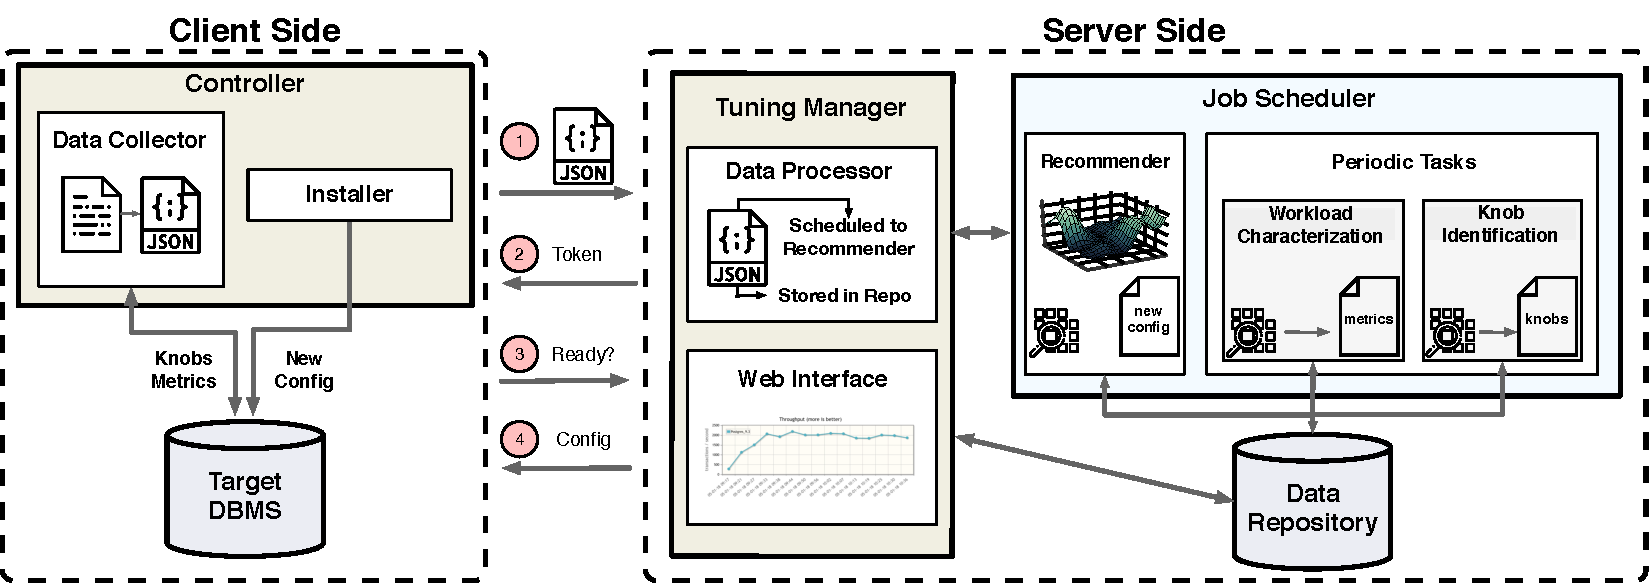
\includegraphics[width=0.95\textwidth]{figures/ottertune-overview.pdf}
    \caption{
        \textbf{\ottertune Architecture Overview} --
        The \toolClient connects to the target DBMS, collects its knob/metric
        data, transforms the collected information into a JSON document, and sends it to the 
        server-side \toolServer.
        The \toolServer stores the information in the data repository and
        schedules a new task with the job scheduler to compute the next
        configuration for the target DBMS to try. The \toolClient (1) sends the 
        information to the \toolServer, (2) gets a token from the \toolServer, (3)
        uses this token to check status of the tuning job, and (4) gets the recommended
        configuration when the job finishes and then the agent installs it in the DBMS.
    }
    \label{fig:ottertune-overview}
\end{figure}

%% ---------------------------------------------------------------
%% Machine Learning Pipeline
%% ---------------------------------------------------------------
\subsection{Machine Learning Pipeline}
\label{sec:ottertune-pipeline}
\ottertune's ML pipeline uses a combination of supervised and unsupervised methods. It processes, 
analyzes, and builds models from the data in its repository. Both the Workload Characterization and 
Knob Identification modules execute as a background task that periodically updates their models 
as new data becomes available in the repository. 
The tuning manager uses these models to generate new knob configurations for the target DBMS.
\ottertune's ML pipeline has three modules: 
\\ \vspace{-0.1in}

%% -----------------------
%% Workload Characterization
%% -----------------------
\textbf{Workload Characterization:}
This first component compresses all of the past metric data
in the repository into a smaller set of metrics that capture the distinguishing characteristics for 
different workloads. It uses \textit{factor analysis} (FA) to model each internal runtime metric as 
linear combinations of a few factors.
It then clusters the metrics via $k$-means, using their factor coefficients as coordinates. Similar 
metrics are in the same cluster, and it selects one representative metric from each cluster, 
namely, the one closest to the cluster's center.
\\ \vspace{-0.1in}

%% -----------------------
%% Knob Identification
%% -----------------------
\textbf{Knob Identification:}
The next component analyzes all past observations in the repository
to determine which knobs have the most impact on the DBMS's performance for different workloads.
\ottertune uses a popular feature-selection technique, called \textit{Lasso}~\cite{hastie01}, to 
determine which knobs have the most impact the system's overall performance.
Lasso is similar to the least-squares model, except that it uses L1 regularization. It forces 
certain coefficients to be set to zero. The larger weight of L1 penalty is, the more coefficients 
become zero.
\\ \vspace{-0.1in}

%% -----------------------
%% Automated Tuner
%% -----------------------
\textbf{Automated Tuner:}
In the last step, the tuner analyzes the results it has collected so far in the tuning session to 
decide which configuration to recommend next. It performs a two-step analysis after each 
observation period. First, the system uses the performance data for the 
metrics identified in the Workload Characterization component to identify the workload from a 
previous tuning session that best represents the target DBMS's workload. It compares the metrics 
collected so far in the tuning session with those from previous workloads by calculating the 
Euclidean distance, and finds the previous workload that is most similar to the target workload, 
namely, the one with smallest Euclidean distance.

%% ==================================================================
%% Self-Driving
%% ==================================================================
\section{\noisepage$ $-- A Self-Driving DBMS Architecture}
\label{sec:selfdriving}
\textbf{\noisepage} is a new DBMS that we are developing at CMU to be 
self-driving~\cite{pavlo17,noisepage}. This means that the system is able to tune and optimize 
itself automatically without any human intervention other than selecting the target objective 
function on start-up. The DBMS's core architecture is a \dbmsPostgres-compatible HTAP system. It 
uses HyPer-style MVCC~\cite{neumann15} over Apache Arrow in-memory 
columnar storage~\cite{li19}.
We chose an in-memory architecture to enable the system to apply actions in minutes (instead of 
hours) with minimal impact on the application's performance. 
Faster action deployment enables the system to quickly explore solutions and collect new training 
data. This enables the system to react better to changes in the application's workload and its 
operating environment. 

% The DBMS is instrumented with a workload and performance monitors that collect information 
% about the entire system. These monitors feed this information to the \textit{modeling} 
% module that trains models that the \textit{planning} module uses to seelectio
% The first part module in the system is a modeling 

The DBMS's control agent runs in a continuous loop where it selects actions to deploy that it 
estimates will improve the target objective. \noisepage supports actions that affect (1) database 
physical design (e.g., add/drop 
indexes), (2) knob configuration (e.g., memory allocation), and (3) hardware resources (e.g., 
scaling up/down). We are not currently investigating how to automatically support query plan tuning 
as these requires more fine-grained models that can reason about individual sessions.

Because the DBMS is built from scratch for autonomous control, we designed the architecture in a 
modular manner to allow agents to collect training data offline more efficiently. That is, one
can start just a single component in the DBMS (e.g., the transaction manager) and then perform 
a parameter sweep across many configurations without having to go through the DBMS's entire 
execution path. This reduces the number of redundant configurations that the system observes 
to (1) improve data collection efficiency and (2) reduce model over-fitting. The DBMS then 
combines this offline data with data collected online during query execution to improve it accuracy.

\begin{figure}[t!]
    \centering
    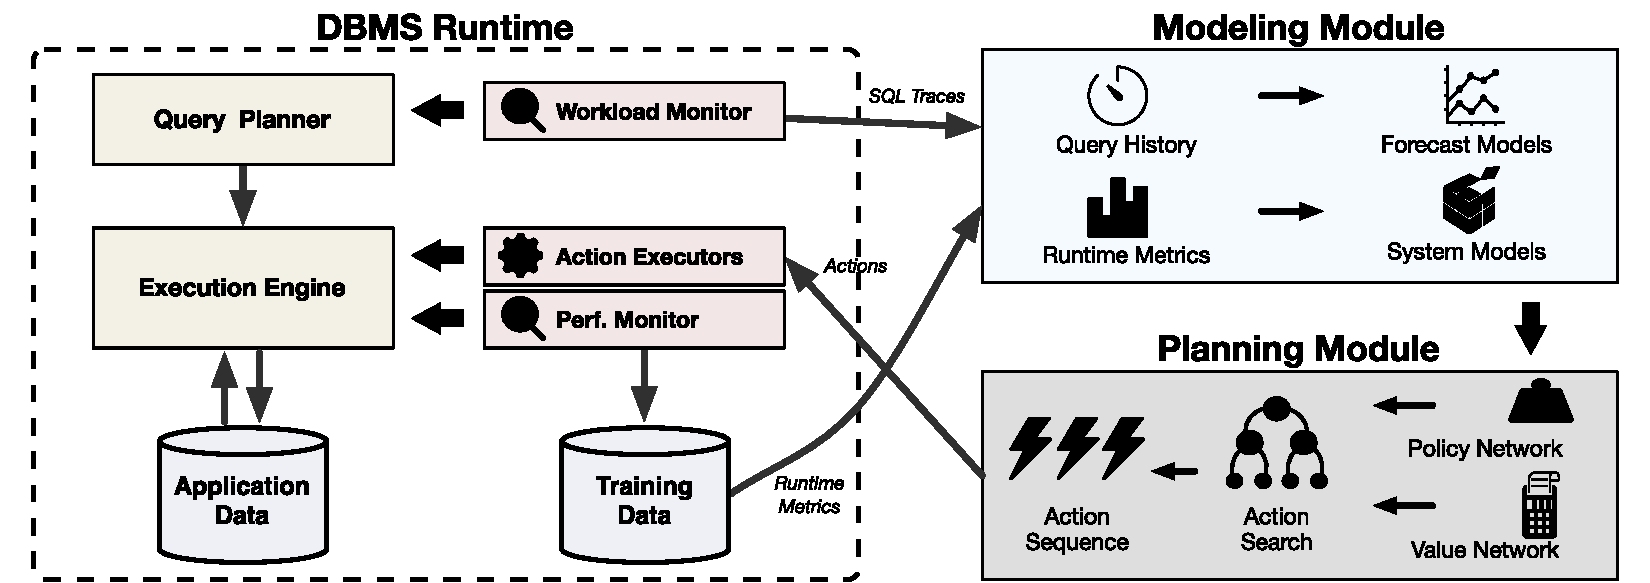
\includegraphics[width=0.95\textwidth]{figures/noisepage-overview.pdf}
    \caption{
        \textbf{\noisepage Architecture Overview} --
        The DBMS contains workload and performance monitors that collect runtime data about the 
        system. It then stores this information in a separate training data repository. The 
        Modeling module retrieves this information and builds forecasting models. These models are 
        then used to guide the Planning module's search process for selecting actions that it 
        believes will improve the DBMS's objective function.
    }
    \label{fig:noisepage-overview}
\end{figure}

%% ---------------------------------------------------------------
%% Machine Learning Pipeline
%% ---------------------------------------------------------------
\subsection{Machine Learning Pipeline}
\label{sec:selfdriving-pipeline}
We next provide an overview of \noisepage's self-driving pipeline. 
Section~\ref{fig:noisepage-overview} illustrates the overall architecture of the DBMS with its modeling 
and planning modules. The DBMS is instrumented with a workload and performance monitors that collect 
information about the entire system during both query execution and action deployment.
\vspace*{-0.1in} \\

%% -----------------------
%% Phase 1
%% -----------------------
\textbf{Modeling:}
This first module is responsible for training prediction models using data that the monitors 
collect from observing its runtime operations. 
There are two categories of models. The first are forecast models that predict the 
application's future workload and database state. 
Forecasting is necessary so that DBMS can prepare itself accordingly, much like a self-driving car 
has to predict the road condition up ahead.
But instead of using cameras and LIDAR like a car, a self-driving DBMS uses workload traces and 
database statistics to generate forecast models~\cite{ma18}. These models are independent of the 
DBMS's configuration since they are determined by the application.
The second category of models predict how the DBMS's internal sub-systems will respond to 
configuration changes made by actions. The DBMS trains these models from its internal metrics 
collected by its performance monitors. It then computes how changes in these models affect the 
target objective function. This is known as the ``value function'' in ML algorithms.
% This training is a continuous process: as the DBMS executes queries and actions, 
% it updates its models to improve their accuracy.
\vspace*{-0.1in} \\

%% -----------------------
%% Phase 2
%% -----------------------
\textbf{Planning:}
In the second module, the DBMS use the models generated in the previous step to select actions 
that provide the best reward (i.e., objective function improvement) given the current state of the 
system. This reward includes an estimation the cost of deploying each action.
The system estimates the application's behavior for some finite prediction horizon using its 
workload forecast models. It then searches for an action that achieves the best reward without 
violating human-defined constraints (e.g., hardware budgets, SLOs).
This search can use either (1) tree-based optimization methods, such as a Monte Carlo search 
tree~\cite{silver16} or (2) RL methods using deep neural networks for policy and value functions. 
The search can be weighted so that it is more likely to consider the actions that provide the most 
benefit for the current state and avoid recently reversed actions.

To avoid having to consider all possible actions at each iteration (e.g., indexes for every 
possible combination of columns), there is a large corpus of previous work on pruning less effective 
or useless actions~\cite{chaudhuri07}. Since the set of relevant candidate actions is dependent on 
the DBMS environment, it can change multiple times during the day. Thus, one key unsolved problem, 
however, is how to represent this dynamic action set in the DBMS's models' fixed-length feature 
vectors.
\vspace*{-0.1in} \\

%% -----------------------
%% Phase 3
%% -----------------------
\textbf{Deployment:}
For a given action selected in the planning module, the next step is for the DBMS to deploy it. 
This part includes the mechanisms to efficiently execute the action's sub-tasks, as well as the 
ability to observe the action's effect on its performance both during and after the 
deployment. The DBMS's planning modules use the data that it collects during this phase 
to update their models and improve their decision making.
% \vspace*{-0.1in} \\

%% ==================================================================
%% CONCLUSION
%% ==================================================================
\section{Conclusion}
\label{sec:conclusion}
Autonomous DBMSs will enable organizations to deploy database applications that are more 
complex than what is possible today, and at a lower cost in terms of both hardware and personnel. 
In this paper, we surveyed the approaches for adding automatic tuning agents based on ML to 
DBMSs. We discussed the high-level differences of external versus and internal agents, as well as 
the separate challenges in these approaches. We then discussed two examples of these architectures 
from CMU: (1) \ottertune~\cite{ottertune} and (2) \noisepage~\cite{noisepage}. Although there is 
still a substantial amount of research needed in both systems and ML before we achieve fully 
autonomous (i.e., self-driving) DBMSs, we contend that the field has made several important steps 
towards this goal in recent years.

One final point that we would like to make is that we believe that autonomous DBMSs will not 
supplant DBAs. We instead envision these systems will emancipate them from the burdens of 
arduous low-level tuning and allow them to pursue higher minded tasks, such as database 
design and development.

%% ==================================================================
%% ACKNOWLEDGEMENTS
%% ==================================================================
\section{Acknowledgments}
\label{sec:ack}

This work was supported (in part) by the National Science Foundation 
%(\href{http://www.nsf.gov/awardsearch/showAward?AWD_ID=1846158}{IIS-1846158}, 
%\href{http://www.nsf.gov/awardsearch/showAward?AWD_ID=1718582}{IIS-1718582},
%\href{http://www.nsf.gov/awardsearch/%showAward?AWD_ID=1822933}{SPX-1822933},
%\href{http://www.nsf.gov/awardsearch/showAward?AWD_ID=1252522}{DGE-1252522}),
%the \href{http://istc-vcs.cmu.edu}
{Intel Science and Technology Center for Visual Cloud Systems},
Google Research Grants, 
AWS Cloud Credits for Research, and the
%\href{https://sloan.org/grant-detail/8638}
{Alfred P. Sloan Research Fellowship} program.


%% ==================================================================
%% BIBLIOGRAPHY
%% ==================================================================
\balance

%\bibliographystyle{abbrv}
%\bibliography{submissions/selfdriving/bulletin}
	
\begin{thebibliography}{10}

\bibitem{cmu-db}
{Carnegie Mellon Database Group}.
\newblock \url{https://db.cs.cmu.edu}.

\bibitem{mysql-tuning-primer}
{MySQL Tuning Primer Script}.
\newblock \url{https://launchpad.net/mysql-tuning-primer}.

\bibitem{noisepage}
{NoisePage}.
\newblock \url{https://noise.page}.

\bibitem{oracle-selfdriving}
{Oracle Self-Driving Database}.
\newblock \url{https://www.oracle.com/database/autonomous-database/index.html}.

\bibitem{ottertune}
{OtterTune}.
\newblock \url{https://ottertune.cs.cmu.edu}.

\bibitem{peloton}
{Peloton}.
\newblock \url{https://pelotondb.io}.

\bibitem{postgres-pgtune}
{PostgreSQL Configuration Wizard}.
\newblock \url{https://pgtune.leopard.in.ua}.

\bibitem{abraham13}
L.~Abraham, J.~Allen, O.~Barykin, V.~Borkar, B.~Chopra, C.~Gerea, D.~Merl,
  J.~Metzler, D.~Reiss, S.~Subramanian, J.~L. Wiener, and O.~Zed.
\newblock Scuba: Diving into data at facebook.
\newblock {\em Proc. VLDB Endow.}, 6(11):1057--1067, Aug. 2013.

\bibitem{arulraj16}
J.~Arulraj, A.~Pavlo, and P.~Menon.
\newblock Bridging the archipelago between row-stores and column-stores for
  hybrid workloads.
\newblock In {\em Proceedings of the 2016 International Conference on
  Management of Data}, SIGMOD '16, pages 583--598, 2016.

\bibitem{bailis17}
P.~Bailis, E.~Gan, S.~Madden, D.~Narayanan, K.~Rong, and S.~Suri.
\newblock Macrobase: Prioritizing attention in fast data.
\newblock In {\em Proceedings of the 2017 ACM International Conference on
  Management of Data}, SIGMOD '17, pages 541--556, 2017.

\bibitem{basu15}
D.~Basu, Q.~Lin, W.~Chen, H.~T. Vo, Z.~Yuan, P.~Senellart, and S.~Bressan.
\newblock {\em Cost-Model Oblivious Database Tuning with Reinforcement
  Learning}, pages 253--268.
\newblock 2015.

\bibitem{bernstein98}
P.~Bernstein, M.~Brodie, S.~Ceri, D.~DeWitt, M.~Franklin, H.~Garcia-Molina,
  J.~Gray, J.~Held, J.~Hellerstein, H.~Jagadish, et~al.
\newblock The asilomar report on database research.
\newblock {\em SIGMOD record}, 27(4):74--80, 1998.

\bibitem{bruno05}
N.~Bruno and S.~Chaudhuri.
\newblock Automatic physical database tuning: a relaxation-based approach.
\newblock In {\em SIGMOD}, pages 227--238, 2005.

\bibitem{ceri83}
S.~Ceri, S.~Navathe, and G.~Wiederhold.
\newblock Distribution design of logical database schemas.
\newblock {\em IEEE Trans. Softw. Eng.}, 9(4):487--504, 1983.

\bibitem{chaudhuri98}
S.~Chaudhuri and V.~Narasayya.
\newblock Autoadmin ``what-if'' index analysis utility.
\newblock {\em SIGMOD Rec.}, 27(2):367--378, 1998.

\bibitem{chaudhuri07}
S.~Chaudhuri and V.~Narasayya.
\newblock Self-tuning database systems: a decade of progress.
\newblock In {\em VLDB}, pages 3--14, 2007.

\bibitem{chaudhuri97}
S.~Chaudhuri and V.~R. Narasayya.
\newblock An efficient cost-driven index selection tool for microsoft {SQL}
  server.
\newblock In {\em VLDB}, pages 146--155, 1997.

\bibitem{chaudhuri00}
S.~Chaudhuri and G.~Weikum.
\newblock Rethinking database system architecture: Towards a self-tuning
  {RISC}-style database system.
\newblock In {\em VLDB}, pages 1--10, 2000.

\bibitem{dageville02}
B.~Dageville and M.~Zait.
\newblock Sql memory management in oracle9i.
\newblock In {\em Proceedings of the 28th International Conference on Very
  Large Data Bases}, VLDB '02, pages 962--973, 2002.

\bibitem{debnath08}
B.~Debnath, D.~Lilja, and M.~Mokbel.
\newblock {SARD}: A statistical approach for ranking database tuning
  parameters.
\newblock In {\em ICDEW}, pages 11--18, 2008.

\bibitem{dias05}
K.~Dias, M.~Ramacher, U.~Shaft, V.~Venkataramani, and G.~Wood.
\newblock Automatic performance diagnosis and tuning in oracle.
\newblock In {\em CIdR}, 2005.

\bibitem{difallah13}
D.~E. Difallah, A.~Pavlo, C.~Curino, and P.~Cudr{\'{e}}{-}Mauroux.
\newblock {OLTP-Bench}: An extensible testbed for benchmarking relational
  databases.
\newblock {\em {PVLDB}}, 7(4):277--288, 2013.

\bibitem{zhang19-ai}
B.~Ding, S.~Das, R.~Marcus, W.~Wu, S.~Chaudhuri, and V.~Narasayya.
\newblock Ai meets ai: Leveraging query executions to improve index
  recommendations.
\newblock In {\em Proceedings of the 2019 ACM International Conference on
  Management of Data}, SIGMOD '19, 2019.

\bibitem{duan09}
S.~Duan, V.~Thummala, and S.~Babu.
\newblock Tuning database configuration parameters with {iTuned}.
\newblock {\em VLDB}, 2:1246--1257, August 2009.

\bibitem{durand18}
G.~C. Durand, M.~Pinnecke, R.~Piriyev, M.~Mohsen, D.~Broneske, G.~Saake, M.~S.
  Sekeran, F.~Rodriguez, and L.~Balami.
\newblock Gridformation: Towards self-driven online data partitioning using
  reinforcement learning.
\newblock aiDM'18, pages 1:1--1:7, 2018.

\bibitem{ganapathi09}
A.~Ganapathi, H.~Kuno, U.~Dayal, J.~L. Wiener, A.~Fox, M.~Jordan, and
  D.~Patterson.
\newblock Predicting multiple metrics for queries: Better decisions enabled by
  machine learning.
\newblock In {\em International Conference on Data Engineering}, pages
  592--603. IEEE, 2009.

\bibitem{graefe14}
G.~Graefe, W.~Guy, and C.~Sauer.
\newblock {\em Instant Recovery with Write-Ahead Logging: Page Repair, System
  Restart, and Media Restore}.
\newblock Synthesis Lectures on Data Management. Morgan {\&} Claypool
  Publishers, 2014.

\bibitem{gupta08}
C.~Gupta, A.~Mehta, and U.~Dayal.
\newblock {PQR: Predicting Query Execution Times for Autonomous Workload
  Management}.
\newblock In {\em ICAC}, pages 13--22, 2008.

\bibitem{gupta97}
H.~Gupta, V.~Harinarayan, A.~Rajaraman, and J.~D. Ullman.
\newblock Index selection for olap.
\newblock In {\em ICDE}, pages 208--219, 1997.

\bibitem{hammer77}
M.~Hammer.
\newblock Self-adaptive automatic data base design.
\newblock In {\em National Computer Conference}, AFIPS '77, pages 123--129,
  1977.

\bibitem{hammer76}
M.~Hammer and A.~Chan.
\newblock Index selection in a self-adaptive data base management system.
\newblock In {\em SIGMOD}, pages 1--8, 1976.

\bibitem{hammer79}
M.~Hammer and B.~Niamir.
\newblock A heuristic approach to attribute partitioning.
\newblock In {\em SIGMOD}, pages 93--101, 1979.

\bibitem{hilprecht19}
B.~Hilprecht, C.~Binnig, and U.~R{\"{o}}hm.
\newblock Towards learning a partitioning advisor with deep reinforcement
  learning.
\newblock In {\em aiDM@SIGMOD}, pages 6:1--6:4, 2019.

\bibitem{hudson89}
S.~E. Hudson and R.~King.
\newblock Cactis: A self-adaptive, concurrent implementation of an
  object-oriented database management system.
\newblock {\em ACM Trans. Database Syst.}, 14(3):291--321, Sept. 1989.

\bibitem{ip83}
M.~Y.~L. Ip, L.~V. Saxton, and V.~V. Raghavan.
\newblock On the selection of an optimal set of indexes.
\newblock {\em IEEE Trans. Softw. Eng.}, 9(2):135--143, 1983.

\bibitem{ivanov17}
O.~Ivanov and S.~Bartunov.
\newblock Adaptive cardinality estimation.
\newblock {\em CoRR}, abs/1711.08330, 2017.

\bibitem{kipf19}
A.~Kipf, T.~Kipf, B.~Radke, V.~Leis, P.~A. Boncz, and A.~Kemper.
\newblock Learned cardinalities: Estimating correlated joins with deep
  learning.
\newblock In {\em {CIDR}}, 2019.

\bibitem{kraska19}
T.~Kraska, M.~Alizadeh, A.~Beutel, E.~H. Chi, A.~Kristo, G.~Leclerc, S.~Madden,
  H.~Mao, and V.~Nathan.
\newblock Sagedb: {A} learned database system.
\newblock In {\em CIDR}, 2019.

\bibitem{kraska18}
T.~Kraska, A.~Beutel, E.~H. Chi, J.~Dean, and N.~Polyzotis.
\newblock The case for learned index structures.
\newblock In {\em Proceedings of the 2018 International Conference on
  Management of Data}, pages 489--504, 2018.

\bibitem{kumar03}
S.~Kumar.
\newblock {Oracle Database 10g}: The self-managing database, Nov. 2003.
\newblock {White Paper}.

\bibitem{kwan02}
E.~Kwan, S.~Lightstone, A.~Storm, and L.~Wu.
\newblock Automatic configuration for {IBM DB2} universal database.
\newblock Technical report, IBM, jan 2002.

\bibitem{ibmdb02}
E.~Kwan, S.~Lightstone, A.~Storm, and L.~Wu.
\newblock Automatic configuration for {IBM DB2} universal database.
\newblock Technical report, IBM, jan 2002.

\bibitem{levin82}
K.~D. Levin.
\newblock Adaptive structuring of distributed databases.
\newblock In {\em National Computer Conference}, AFIPS '82, pages 691--696,
  1982.

\bibitem{li19}
T.~Li, M.~Butrovich, A.~Ngom, W.~McKinney, and A.~Pavlo.
\newblock Mainlining databases: Supporting fast transactional workloads on
  universal columnar data file formats.
\newblock 2019.
\newblock \textit{Under Submission}.

\bibitem{liu15}
H.~Liu, M.~Xu, Z.~Yu, V.~Corvinelli, and C.~Zuzarte.
\newblock Cardinality estimation using neural networks.
\newblock CASCON '15, pages 53--59, 2015.

\bibitem{ma18}
L.~Ma, D.~V. Aken, A.~Hefny, G.~Mezerhane, A.~Pavlo, and G.~J. Gordon.
\newblock Query-based workload forecasting for self-driving database management
  systems.
\newblock In {\em Proceedings of the 2018 ACM International Conference on
  Management of Data}, SIGMOD '18, 2018.

\bibitem{marcus19}
R.~Marcus, P.~Negi, H.~Mao, C.~Zhang, M.~Alizadeh, T.~Kraska, O.~Papaemmanouil,
  and N.~Tatbul.
\newblock Neo: {A} learned query optimizer.
\newblock {\em CoRR}, abs/1904.03711, 2019.

\bibitem{marcus18}
R.~Marcus and O.~Papaemmanouil.
\newblock Deep reinforcement learning for join order enumeration.
\newblock In {\em aiDM@SIGMOD}, pages 3:1--3:4, 2018.

\bibitem{marcus19-perf}
R.~Marcus and O.~Papaemmanouil.
\newblock Plan-structured deep neural network models for query performance
  prediction.
\newblock {\em CoRR}, abs/1902.00132, 2019.

\bibitem{marcus19-opt}
R.~Marcus and O.~Papaemmanouil.
\newblock Towards a hands-free query optimizer through deep learning.
\newblock In {\em {CIDR} 2019, 9th Biennial Conference on Innovative Data
  Systems Research}, 2019.

\bibitem{mozafari13}
B.~Mozafari, C.~Curino, A.~Jindal, and S.~Madden.
\newblock Performance and resource modeling in highly-concurrent oltp
  workloads.
\newblock In {\em Proceedings of the 2013 ACM SIGMOD International Conference
  on Management of Data}, SIGMOD '13, pages 301--312, 2013.

\bibitem{mukkamala88}
R.~Mukkamala, S.~C. Bruell, and R.~K. Shultz.
\newblock Design of partially replicated distributed database systems: an
  integrated methodology.
\newblock {\em SIGMETRICS Perform. Eval. Rev.}, 16(1):187--196, 1988.

\bibitem{narayanan05}
D.~Narayanan, E.~Thereska, and A.~Ailamaki.
\newblock Continuous resource monitoring for self-predicting {DBMS}.
\newblock In {\em MASCOTS}, pages 239--248, 2005.

\bibitem{nehme11}
R.~Nehme and N.~Bruno.
\newblock Automated partitioning design in parallel database systems.
\newblock In {\em SIGMOD}, SIGMOD, pages 1137--1148, 2011.

\bibitem{neumann15}
T.~Neumann, T.~M{\"u}hlbauer, and A.~Kemper.
\newblock Fast serializable multi-version concurrency control for main-memory
  database systems.
\newblock SIGMOD, 2015.

\bibitem{ortiz18}
J.~Ortiz, M.~Balazinska, J.~Gehrke, and S.~S. Keerthi.
\newblock Learning state representations for query optimization with deep
  reinforcement learning.
\newblock DEEM'18, pages 4:1--4:4, 2018.

\bibitem{pavlo17}
A.~Pavlo, G.~Angulo, J.~Arulraj, H.~Lin, J.~Lin, L.~Ma, P.~Menon, T.~Mowry,
  M.~Perron, I.~Quah, S.~Santurkar, A.~Tomasic, S.~Toor, D.~V. Aken, Z.~Wang,
  Y.~Wu, R.~Xian, and T.~Zhang.
\newblock Self-driving database management systems.
\newblock In {\em {CIDR} 2017, Conference on Innovative Data Systems Research},
  2017.

\bibitem{pavlo12}
A.~Pavlo, C.~Curino, and S.~Zdonik.
\newblock {Skew-Aware Automatic Database Partitioning in Shared-Nothing,
  Parallel OLTP Systems}.
\newblock In {\em SIGMOD}, pages 61--72, 2012.

\bibitem{pavlo19}
A.~Pavlo et~al.
\newblock {Make Your Database Dream of Electric Sheep: Engineering for
  Self-Driving Operation}.
\newblock 2019.
\newblock \textit{Under Submission}.

\bibitem{pavlo11}
A.~Pavlo, E.~P. Jones, and S.~Zdonik.
\newblock On predictive modeling for optimizing transaction execution in
  parallel oltp systems.
\newblock {\em Proc. VLDB Endow.}, 5:85--96, October 2011.

\bibitem{sculley14}
D.~Sculley, G.~Holt, D.~Golovin, E.~Davydov, T.~Phillips, D.~Ebner,
  V.~Chaudhary, and M.~Young.
\newblock Machine learning: The high interest credit card of technical debt.
\newblock In {\em SE4ML: Software Engineering for Machine Learning (NIPS 2014
  Workshop)}, 2014.

\bibitem{sharma18}
A.~Sharma, F.~M. Schuhknecht, and J.~Dittrich.
\newblock The case for automatic database administration using deep
  reinforcement learning.
\newblock {\em CoRR}, abs/1801.05643, 2018.

\bibitem{sheng19}
Y.~Sheng, A.~Tomasic, T.~Zhang, and A.~Pavlo.
\newblock Scheduling {OLTP} transactions via learned abort prediction.
\newblock In {\em aiDM@SIGMOD}, pages 1:1--1:8, 2019.

\bibitem{silver16}
D.~Silver, A.~Huang, C.~J. Maddison, A.~Guez, L.~Sifre, G.~van~den Driessche,
  J.~Schrittwieser, I.~Antonoglou, V.~Panneershelvam, M.~Lanctot, S.~Dieleman,
  D.~Grewe, J.~Nham, N.~Kalchbrenner, I.~Sutskever, T.~Lillicrap, M.~Leach,
  K.~Kavukcuoglu, T.~Graepel, and D.~Hassabis.
\newblock Mastering the game of go with deep neural networks and tree search.
\newblock {\em Nature}, 529:484--503, 2016.

\bibitem{soror08}
A.~A. Soror, U.~F. Minhas, A.~Aboulnaga, K.~Salem, P.~Kokosielis, and
  S.~Kamath.
\newblock Automatic virtual machine configuration for database workloads.
\newblock In {\em SIGMOD}, pages 953--966, 2008.

\bibitem{stillger01}
M.~Stillger, G.~M. Lohman, V.~Markl, and M.~Kandil.
\newblock {LEO - DB2's LEarning Optimizer}.
\newblock In {\em Proceedings of the 27th International Conference on Very
  Large Data Bases}, VLDB '01, pages 19--28, 2001.

\bibitem{storm06}
A.~J. Storm, C.~Garcia-Arellano, S.~S. Lightstone, Y.~Diao, and M.~Surendra.
\newblock Adaptive self-tuning memory in {DB2}.
\newblock In {\em VLDB}, pages 1081--1092, 2006.

\bibitem{sullivan04}
D.~G. Sullivan, M.~I. Seltzer, and A.~Pfeffer.
\newblock Using probabilistic reasoning to automate software tuning.
\newblock SIGMETRICS, pages 404--405, 2004.

\bibitem{hastie01}
T.Hastie, R.Tibshirani, and J.Friedman.
\newblock {\em The Elements of Statistical Learning}.
\newblock Springer, 2001.

\bibitem{tian03}
W.~Tian, P.~Martin, and W.~Powley.
\newblock Techniques for automatically sizing multiple buffer pools in {DB2}.
\newblock In {\em CASCON}, pages 294--302, 2003.

\bibitem{valentin00}
G.~Valentin, M.~Zuliani, D.~Zilio, G.~Lohman, and A.~Skelley.
\newblock {DB2} advisor: an optimizer smart enough to recommend its own
  indexes.
\newblock In {\em ICDE}, pages 101--110, 2000.

\bibitem{vanaken17}
D.~Van~Aken, A.~Pavlo, G.~J. Gordon, and B.~Zhang.
\newblock Automatic database management system tuning through large-scale
  machine learning.
\newblock In {\em Proceedings of the 2017 ACM International Conference on
  Management of Data}, SIGMOD '17, pages 1009--1024, 2017.

\bibitem{weikum94}
G.~Weikum, C.~Hasse, A.~M\"{o}nkeberg, and P.~Zabback.
\newblock The {COMFORT} automatic tuning project.
\newblock {\em Information Systems}, 19(5):381--432, July 1994.

\bibitem{weikum02}
G.~Weikum, A.~Moenkeberg, C.~Hasse, and P.~Zabback.
\newblock Self-tuning database technology and information services: From
  wishful thinking to viable engineering.
\newblock In {\em Proceedings of the 28th International Conference on Very
  Large Data Bases}, VLDB '02, pages 20--31, 2002.

\bibitem{wiese08}
D.~Wiese, G.~Rabinovitch, M.~Reichert, and S.~Arenswald.
\newblock Autonomic tuning expert: A framework for best-practice oriented
  autonomic database tuning.
\newblock In {\em Proceedings of the 2008 Conference of the Center for Advanced
  Studies on Collaborative Research: Meeting of Minds}, CASCON '08, pages
  3:27--3:41, 2008.

\bibitem{woltmann19}
L.~Woltmann, C.~Hartmann, M.~Thiele, D.~Habich, and W.~Lehner.
\newblock Cardinality estimation with local deep learning models.
\newblock In {\em aiDM@SIGMOD}, pages 5:1--5:8, 2019.

\bibitem{xi04}
B.~Xi, Z.~Liu, M.~Raghavachari, C.~H. Xia, and L.~Zhang.
\newblock A smart hill-climbing algorithm for application server configuration.
\newblock In {\em WWW}, pages 287--296, 2004.

\bibitem{yu85}
C.~T. Yu, C.-m. Suen, K.~Lam, and M.~K. Siu.
\newblock Adaptive record clustering.
\newblock {\em ACM Trans. Database Syst.}, 10(2):180--204, June 1985.

\bibitem{zhang18-ottertune}
B.~Zhang, D.~V. Aken, J.~Wang, T.~Dai, S.~Jiang, J.~Lao, S.~Sheng, A.~Pavlo,
  and G.~J. Gordon.
\newblock A demonstration of the ottertune automatic database management system
  tuning service.
\newblock {\em {PVLDB}}, 11(12):1910--1913, 2018.

\bibitem{zhang19-cdbtune}
J.~Zhang, Y.~Liu, K.~Zhou, G.~Li, Z.~Xiao, B.~Cheng, J.~Xing, Y.~Wang,
  T.~Cheng, L.~Liu, M.~Ran, and Z.~Li.
\newblock An end-to-end automatic cloud database tuning system using deep
  reinforcement learning.
\newblock In {\em Proceedings of the 2019 ACM International Conference on
  Management of Data}, SIGMOD '19, 2019.

\bibitem{zhang18-icde}
T.~Zhang, A.~Tomasic, Y.~Sheng, and A.~Pavlo.
\newblock Performance of {OLTP} via intelligent scheduling.
\newblock In {\em ICDE}, pages 1288--1291, 2018.

\bibitem{zilio04}
D.~C. Zilio, J.~Rao, S.~Lightstone, G.~Lohman, A.~Storm, C.~Garcia-Arellano,
  and S.~Fadden.
\newblock {DB2} design advisor: integrated automatic physical database design.
\newblock In {\em VLDB}, pages 1087--1097, 2004.

\end{thebibliography}


\end{document}

